\documentclass{amsart}

\newtheorem{theorem}{Theorem}[section]
\newtheorem{lemma}[theorem]{Lemma}

\theoremstyle{definition}
\newtheorem{definition}[theorem]{Definition}
\newtheorem{example}[theorem]{Example}
\newtheorem{xca}[theorem]{Exercise}

\theoremstyle{remark}
\newtheorem{remark}[theorem]{Remark}

\numberwithin{equation}{section}

% Some packages
\usepackage{listings, color, keyval}

% Some commands
\newcommand{\RR}{\mathbb{R}}
\newcommand{\NN}{\mathbb{N}}
\newcommand{\CC}{\mathbb{C}}
\newcommand{\II}{\mathbb{I}}
\newcommand{\KK}{\mathbb{K}}


%%% Florian

\newcommand{\Id}{\mathrm{Id}}
\renewcommand{\vec}{\textbf}
\usepackage{graphicx}
\usepackage[left=2cm,right=2cm,top=2.6cm,bottom=1.4cm,includefoot]{geometry}


\begin{document}

\title{Iterative Methods}

%    author information
\author{Thanh-Van Huynh, Michael Thiele, Florian Wolf}
\email{thanh-van.huynh@uni-konstanz.de, michael.thiele@uni-konstanz.de, florian.2.wolf@uni-konstanz.de}

%\dedicatory{Thanks Gabriele and Christian for your great work.}

\begin{abstract}
	This is a report about the findings of Thanh-Van Huynh, Michael Thiele and Florian Wolf in the exercises accompanying Iterative Methods for Linear Systems. The lecture was held by Jun.-Prof. Dr. Gabriele Ciaramella with the assistance of Christian Jäckle in the winter term 2020/21 at the University of Constance.
\end{abstract}

\maketitle

\tableofcontents


%% ====================================================================

\section{Introduction}
In the exercises we studied optimal control problems governed by the Laplace equation. We want to solve
\begin{equation*}
\min\limits_{\underline{y},\underline{u}\in\Omega} J(\underline{y},\underline{u}) := \frac{1}{2}\ ||\underline{y}-\underline{y_d}||_{L^2(\Omega)}^2 + \frac{\nu}{2}\ ||\underline{u}||_{L^2(\Omega)}^2
\end{equation*}
with norm
\begin{equation*}
||\underline{x}||_{L^2(\Omega)}^2 := h^2 \sum\limits_{j=1}^n \underline{x}_j^2
\end{equation*}
such that
\begin{equation*}
A\underline{y}=\underline{f}+\underline{u}
\end{equation*}
with $\nu>0$ is satisfied. Notice that we do not have any boundary conditions. One possible way of finding a solution is the so-called reduced approach: We consider $\underline{y}$ as a function of $\underline{u}$, therefore obtaining the problem
\begin{equation*}
\min\limits_{\underline{u}\in\Omega} \hat{J}(\underline{u}) := J(\underline{y}(\underline{u}),\underline{u}).
\end{equation*}

%% ====================================================================

\section{Stationary Methods}
\subsection{Deriving the Optimality System}
We see that
\begin{equation*}
||\underline{x}||_{L^2(\Omega)}^2 = h^2\ ||\underline{x}||_2^2
\end{equation*}
holds for arbitrary $x$. In combination with $\underline{y}=A^{-1}\left(\underline{f}+\underline{u}\right)$, we obtain
\begin{flalign*}
\min\limits_{\underline{u}\in\Omega} \hat{J}(\underline{u}) 
&=\ \frac{1}{2}\ h^2 ||A^{-1}\left(\underline{f}+\underline{u}\right)-\underline{y_d}||_2^2\ + \frac{\nu}{2}\ h^2 ||\underline{u}||_2^2\\
& =\ \frac{1}{2}\ h^2 \langle A^{-1}\left(\underline{f}+\underline{u}\right)-\underline{y_d},A^{-1}\left(\underline{f}+\underline{u}\right)-\underline{y_d}\rangle + \frac{\nu}{2}\ h^2 \langle\underline{u},\underline{u}\rangle\\
& =\ \frac{1}{2}\ h^2  \left(A^{-1}\left(\underline{f}+\underline{u}\right)-\underline{y_d}\right)^{\top} \left(A^{-1}\left(\underline{f}+\underline{u}\right)-\underline{y_d}\right) + \frac{\nu}{2}\ h^2 \underline{u}^{\top}\underline{u}.
\end{flalign*}
As we know that a solution $\underline{u}$ to the problem above has to satisfy $\nabla\hat{J}(\underline{u})=0$, this results in
\begin{equation*}
\nabla \hat{J}(\underline{u}) = h^2 A^{-1} \left(A^{-1} (\underline{f}+\underline{u})-\underline{y_d}\right) + \nu h^2\underline{u} = 0.
\end{equation*}
We can do the following transformations
\begin{flalign*}
h^2 A^{-1} \left(A^{-1} (\underline{f}+\underline{u})-\underline{y_d}\right) + \nu h^2\underline{u} &= 0\\
A^{-1} \left(A^{-1} (\underline{f}+\underline{u})-\underline{y_d}\right) + \nu \underline{u} &=0\\
A^{-1} A^{-1} (\underline{f}+\underline{u})-A^{-1}\underline{y_d} + \nu \underline{u} &=0\\
A^{-1} A^{-1} \underline{f}+A^{-1} A^{-1}\underline{u}-A^{-1}\underline{y_d} + \nu \underline{u} &=0\\
A^{-1} A^{-1} \underline{u} + \nu \underline{u} &=A^{-1}\underline{y_d}-A^{-1} A^{-1}\underline{f}\\
\left(\nu\text{I}+A^{-1} A^{-1}\right) \underline{u} &=A^{-1}\left(\underline{y_d}-A^{-1}\underline{f}\right)
\end{flalign*}
and derive the optimality system
\begin{equation}
\left(\nu\text{I}+A^{-2}\right) \underline{u} =A^{-1}\left(\underline{y_d}-A^{-1}\underline{f}\right) \label{eq:normalOptimalitySystem}
\end{equation}
or alternatively
\begin{equation}
\left(A^2\nu+\text{I}\right) \underline{u} =A\underline{y_d}-\underline{f}. \label{eq:factoredOptimalitySystem}
\end{equation}

%% ====================================================================

\subsection{Laplace Matrices}
First, we implement a function \texttt{FD\_Laplacian} to create the Finite Difference matrix representation of the Laplace operator in sparse.
Depending on whether we choose $d=1$ or $d=2$, we obtain the 1D Laplace Matrix 
$$ T_1 = 
\begin{pmatrix}
-2 & 1 & & & \\
1 & -2 & 1 & & \\
& \ddots & \ddots & \ddots & \\
%& & \ddots & \ddots & 1 \\
%& & & 1 & -2  
\end{pmatrix} \in\RR^{m\times m}
$$
or the 2D Laplace Matrix (by using the Kronecker product $\otimes$)
$$ T_2 = \text{I}_m \otimes T_1 + T_1 \otimes \text{I}_m= 
\begin{pmatrix}
T_1 & \text{I}_m & & \\
\text{I}_m & T_1 & \text{I}_m & \\
& \ddots & \ddots & \ddots
\end{pmatrix} \in\RR^{m^2\times m^2}.
$$

\begin{lstlisting}[mathescape, language=Pascal, title=FD\_Laplacian,
frame=single, numbers=left, numberstyle=\tiny, tabsize=2,
morekeywords={Enter, Return, elif}, deletekeywords={of,or}, keywordstyle=\bfseries]{}
Enter: matrix dimension $m\in\NN$, $d=\{1,2\}$ choosing 1D or 2D
Return: Laplace matrix $T\in\RR^{m\times m}$
diag = -2*sparse.identity($m$)
onesUpper = sparse.eye($m,k=1$)
onesLower = sparse.eye($m,k=-1$)
$T$ = diag + onesUpper + onesLower
if $d==2$:
	eye = sparse.eye($m$)
	$T$ = sparse.kron(eye,$T$) + sparse.kron($T$,eye)
return($T$)
\end{lstlisting}

%% ====================================================================

\subsection{Fast Poisson Solver}
Now, we implement the Fast Poisson Solver \texttt{Fast\_Poisson} to efficiently solve a linear system $Au=b$. As we do not have any boundary conditions, we have a simpler implementation:

\begin{lstlisting}[mathescape, language=Pascal, title=Fast\_Poisson,
frame=single, numbers=left, numberstyle=\tiny, tabsize=2,
morekeywords={Enter, Return, elif}, deletekeywords={of}, keywordstyle=\bfseries]{}
Enter: matrix $V$ of eigenvectors of the matrix $A\in\RR^{m\times m}$, 
vector $\lambda$ of eigenvalues of the matrix $A$, 
right-hand side $b$ of the linear system
Return: solution $u$ of the linear system $Au=b$
$B$ = reshape($b,(m,m)$)
$\tilde{B} = (V^{\top}(V^{\top}B)^{\top})^{\top}$
for i in 0:m
	for j in 0:m
			$\tilde{u}_{ij}=(\tilde{B}_{i,j})/(\lambda_i+\lambda_j)$
$U = (V(V\tilde{U})^{\top})^{\top}$
$u$ = reshape($U,m^2$)
return($u$)
\end{lstlisting}

%% ====================================================================

\subsection{Convergence Analysis}
Now, we solve the system (\ref{eq:normalOptimalitySystem}) by the stationary iteration
\begin{equation}
\underline{u}^{n+1} = -\frac{1}{\nu} A^{-2}\underline{u}^n + \frac{1}{\nu} A^{-1} (\underline{y}_d-A^{-1}\underline{f})
\end{equation}
and analyze its convergence behavior for different $m$ and $\nu$.

%% ====================================================================

\subsection{Damped Jacobi}

%% ====================================================================

\section{Krylov Methods}
In this part of the project we want to use the fact that the matrix arising in our disretization is symmetric and positive definite. For this reason we want to apply the conjugated gradient (CG) method, to solve our systems \eqref{eq:normalOptimalitySystem} and \eqref{eq:factoredOptimalitySystem}.
For the first system we use the already implemented fast poisson solver, to get a matrix free version of the system. In the second case we construct our sparse matrices and use the \texttt{scipy.sparse.linalg.LinearOperator} method, to create a linear operator of our left hand side of the equation.
Looking at the plots below, we can see the following convergence behaviour for the both systems. In the plots $\nu$ ist getting bigger going from top to bottom and $m$ is getting bigger going from left to right.
\begin{figure}[h!]
\centering
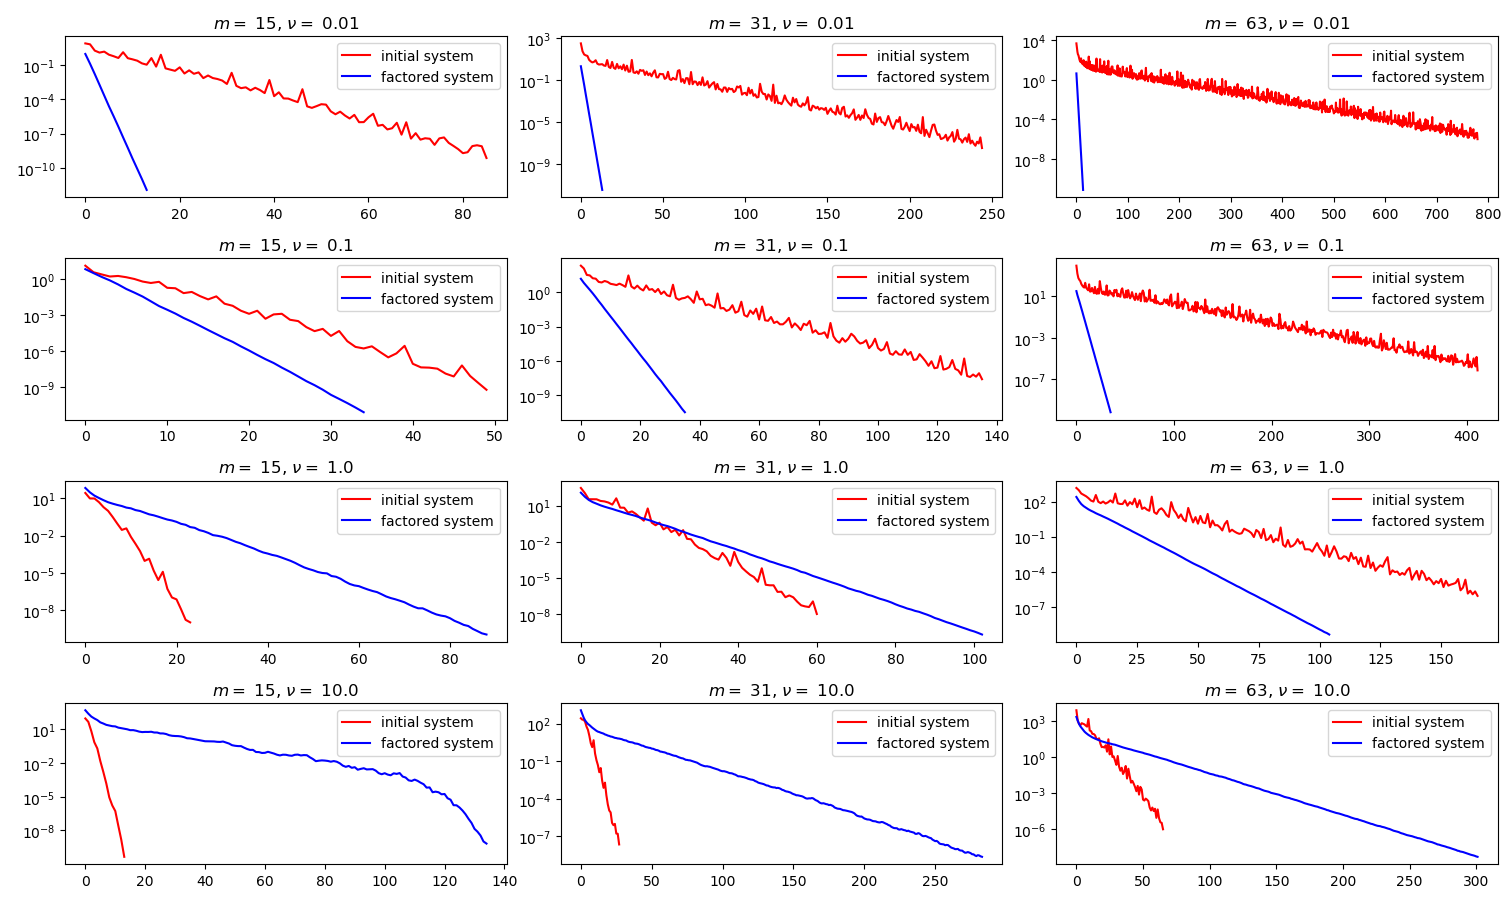
\includegraphics[scale=0.37]{./imgs/CG_analysis}
\caption{Convergence behaviour for different values of $m$ and $\nu$}
\end{figure}
%% ====================================================================

\subsection{Convergence Analysis}

%% ====================================================================

\subsection{Conditional Number}

%% ====================================================================

\section{Multigrid}

%% ====================================================================

\subsection{Stationary Method as Smoother}

%% ====================================================================

\subsection{Damped Jacobi as Smoother}
aoishdjfkljashgkfj
\end{document}

